\begin{flushleft}
\subsection{Use-case diagram}
Vi startede med at lavet et use-case diagram, da dette er en central del af analysefase. Et use-case diagram viser det forskellige ting Player interagere med Matador spillet. Det diagram vi har udarbejdet kan man se at en Player kan "Play Matador", og til denne use-case er der nogle sub use-cases som er Start Game, Buy House or Hotel, Sell House or Hotel, Pawn Property, Buyback Pawned Property, Buy property or auction and Roll Dice. 
\begin{figure}[htp]
    \centering
    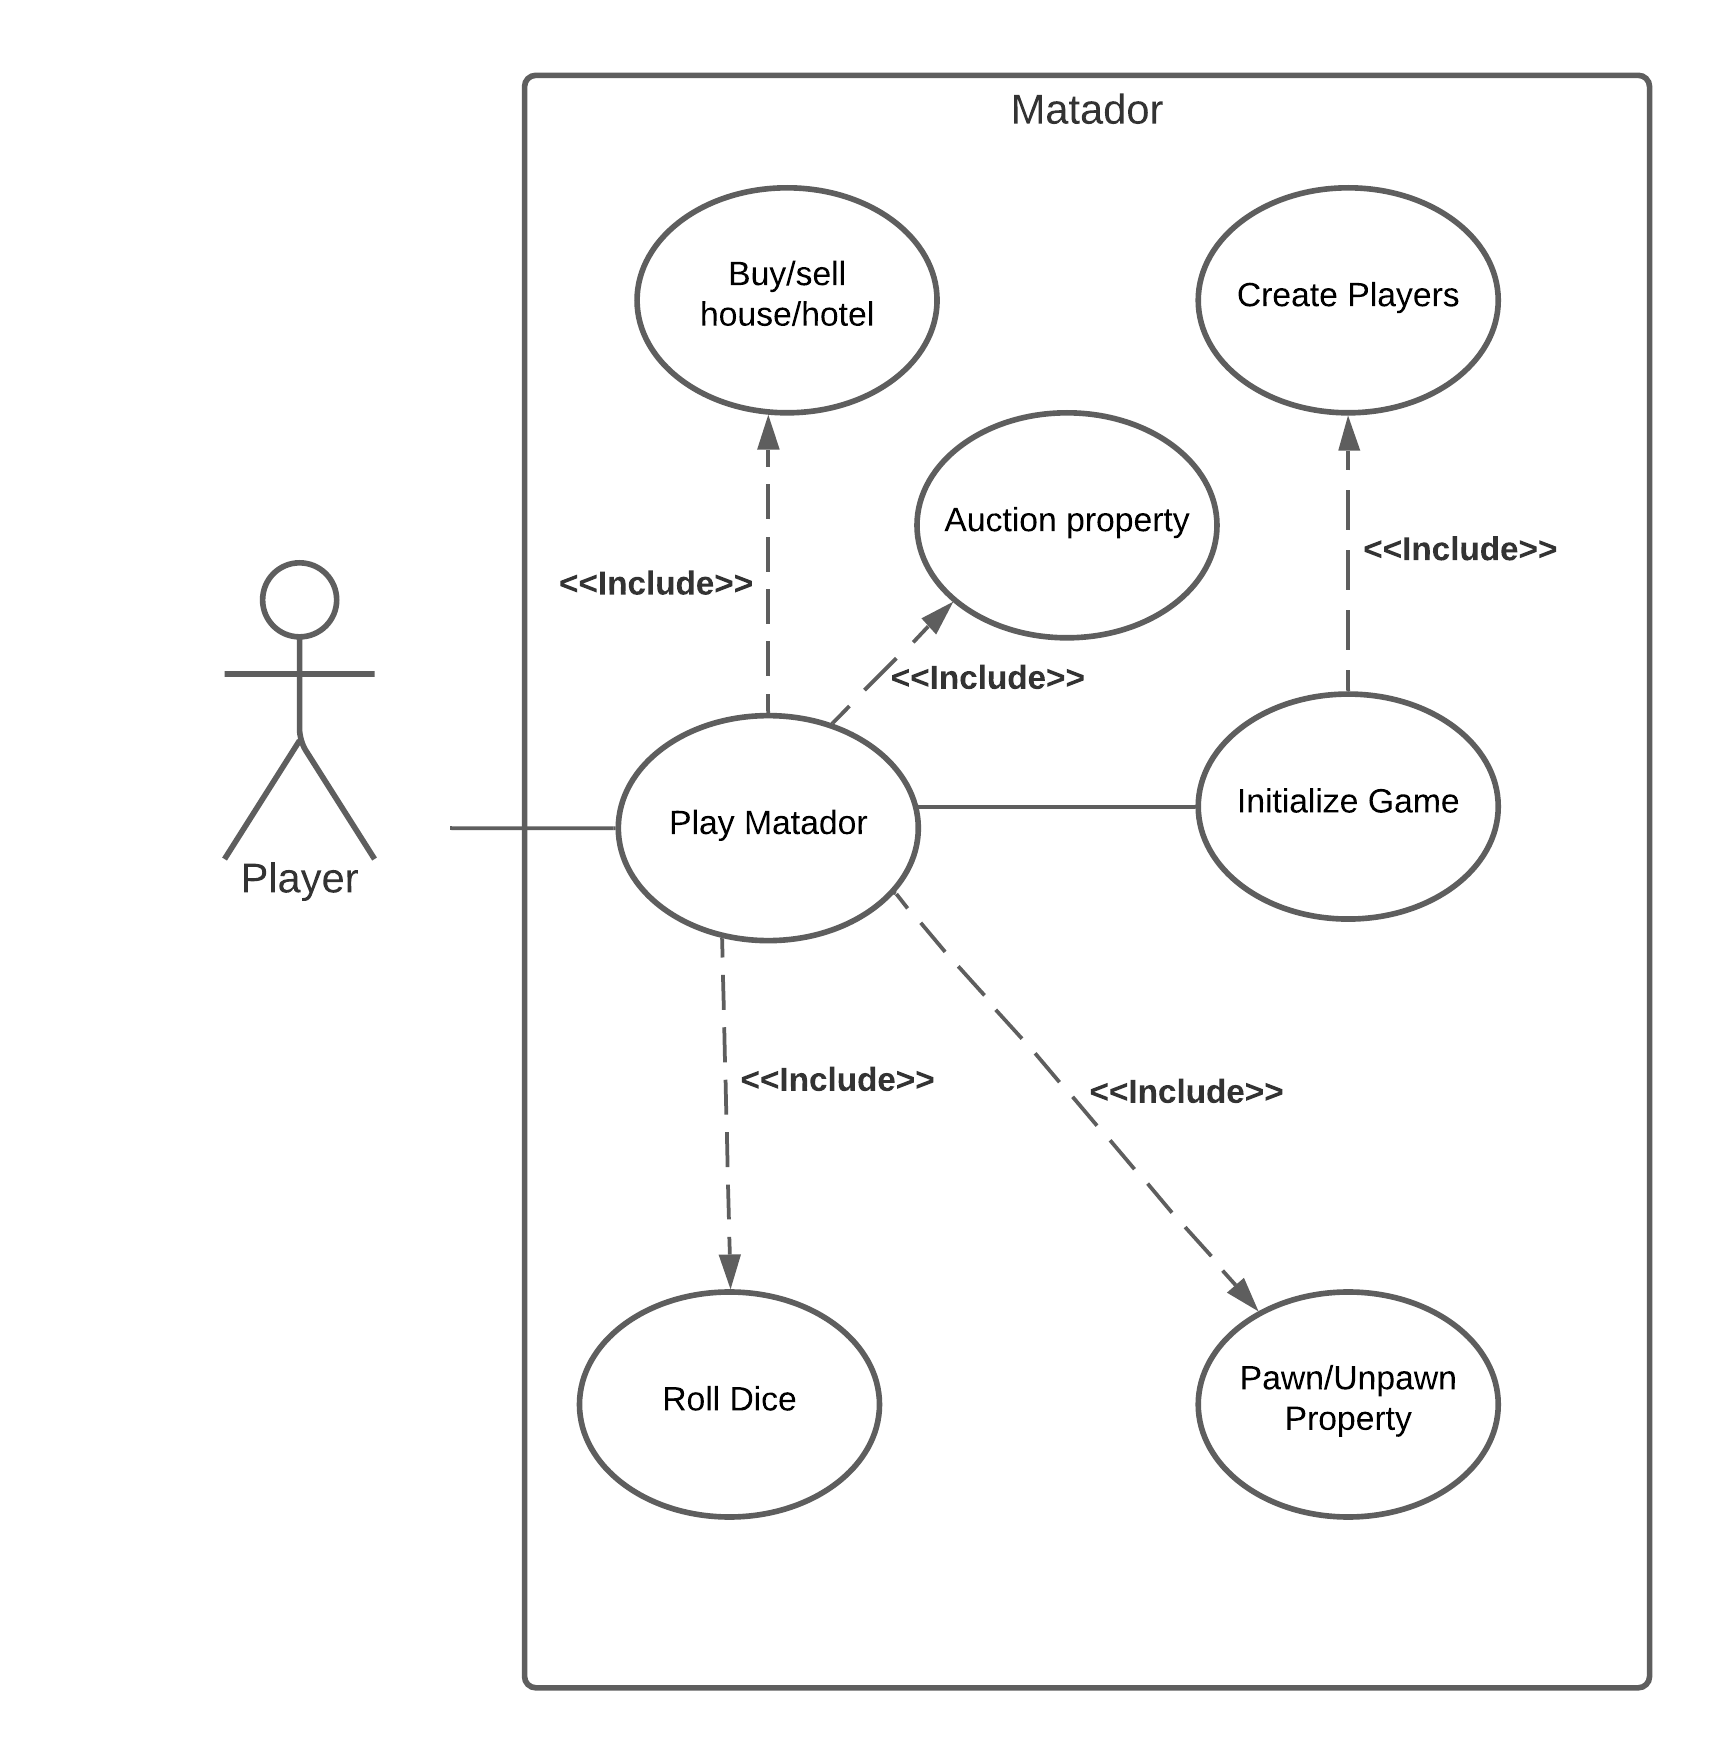
\includegraphics[width=12cm]{Report/figures/Use Case Diagram.png}
    \caption{Use-case diagram}
\end{figure}

\subsection{Central use-case: Roll dice}
Her under er en fully dressed beskrivelse af vores centrale use.case, Roll Dice. \\
\begin{figure}[htp]
    \centering
\begin{tabular}{ |c|c|c|c|c|c|  }
\hline
\multicolumn{2}{|c|}{Fully dressed use-case} \\
\hline
Use-case section & Comment \\
\hline
Use-case Name & Roll dice\\
\hline
Scope & Matador Game\\
\hline
Level & User Goal\\
\hline
Stakeholders and Interests & Players\\
\hline
Preconditions & Player chooses the GUI option to roll dice.\\
\hline
Postconditions & Game changes to next player.\\
\hline
Main success scenario & 1. Player rolls dice.\\
                      & 2. Dice values are shown on the GUI.\\
                    & 3. Player object moves on the GUI gameboard\\
                    & according to the sum of dice facevalue.\\
                    & 4. The gameboard field landed on \\
                    & executes its corresponding actions.\\
                    & 5. Current player's turn ends.\\
                    & 6. Game changes to next player.\\
\hline
Extensions & 6a. One player wins the game. \\
                   & 1. Winner is displayed.\\
                   & 2. Game exits.       \\
                   & 6b. A player rolls identical dices. \\
                   & 1. Steps 2 through 4 in Main success scenario\\
                   & are executed, but player can roll dice again. \\
                   & 1a. Player rolls identical dices thrice in a row.\\
                   & 1. Player moves to jail field on gameboard. \\
                   & 2. Continues from step 5 in Main success scenario.\\
\hline
Special Requirements & Arbitrary.\\
\hline
Technology and Data Variations list & N/A.\\
\hline
Frequency of Occurrence & Continuous.\\
\hline
Misc. & N/A.\\
\hline

    \end{tabular}\\
    \caption{Fully dressed use-case af roll dice use-case.}
\end{figure}
\doublespacing

\subsection{Sub use-cases}
Her er vores liste over use-cases.\\
\begin{figure}[htp]
    \centering
\begin{tabular}{ |c|c|c|c|c|c|  }
\hline
\multicolumn{2}{|c|}{Brief use-case} \\
\hline
Use-case & A short use case description \\
\hline
Start Game & Spillet starter med at man skal vælge \\
&hvor mange spiller der skal være med.\\
&Herefter indtaster hver spiller deres navn og den\\
&første spiller som indtaster deres navn starter.\\
\hline
Buy House or Hotel & I starten af spillerens tur får spilleren mulighed\\
&for at køber huse eller hoteller.\\
\hline
Sell House or Hotel & I starten af spillerens tur får spilleren mulighed\\
&for at sælge huse eller hoteller.\\
\hline
Pawn Property & Spilleren har mulighed for at pantsætte \\
&sine grunde i starten af turen.\\
\hline
Buyback Pawned Property & Spilleren har mulighed for at tilbage købe\\
&pantsætte grunde i starten af turen.\\
\hline
Buy Property or Auction & Hvis man lander på en grund for man \\
&mulighed for at købe den, men hvis man ikke\\
&gider eller kan købe grunden bilver den\\
&sat til salg på aution hvor alle kan deltage\\
\hline


    \end{tabular} \\
    \caption{Brief use-cases}
\end{figure}
\doublespacing


\subsection{Domæne model}
Det centrale objekt i domæne modelen er MatadorGame. Det indholder mellem 2 til 6 Player, 46 ChanceCard, 2 Dice og en Field. Til hver Player som bliver opretter bliver der også oprettet en Account, som bliver påvirket af Field. Field har også JailField, ChanceField, CustomField, PropertyField, StartField, TaxField, SodaField and FerryField.
\begin{figure}[htp]
    \centering
    \includegraphics[width=16cm]{Report/figures/Domæne model.png}
    \caption{Domæne model}
\end{figure}

\subsection{Systemsekvensdiagram}
Her til at afrund vores analysedel hvor vi har udarbejdet et systemsekvensdiagram over Matador spillet. Systemsekvensdiagram viser Player og interaktion med Matador spillet. 
\begin{figure}[htp]
    \centering
    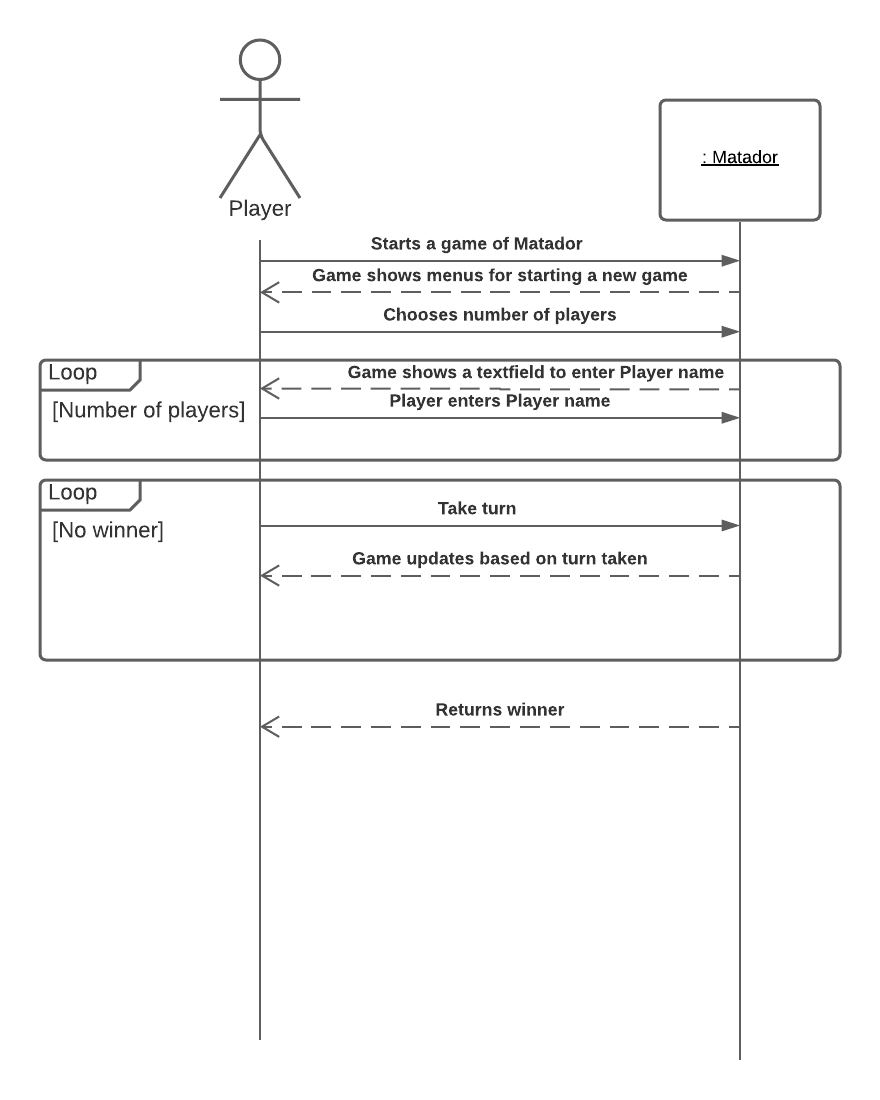
\includegraphics[width=13cm]{Report/figures/System Sekvens Diagram.png}
    \caption{Systemsekvensdiagram}
\end{figure}

\end{flushleft}